\subsection{Casa Familia}

\begin{figure}[H]
	\center
	\begin{subfigure}{0.4\textwidth}
		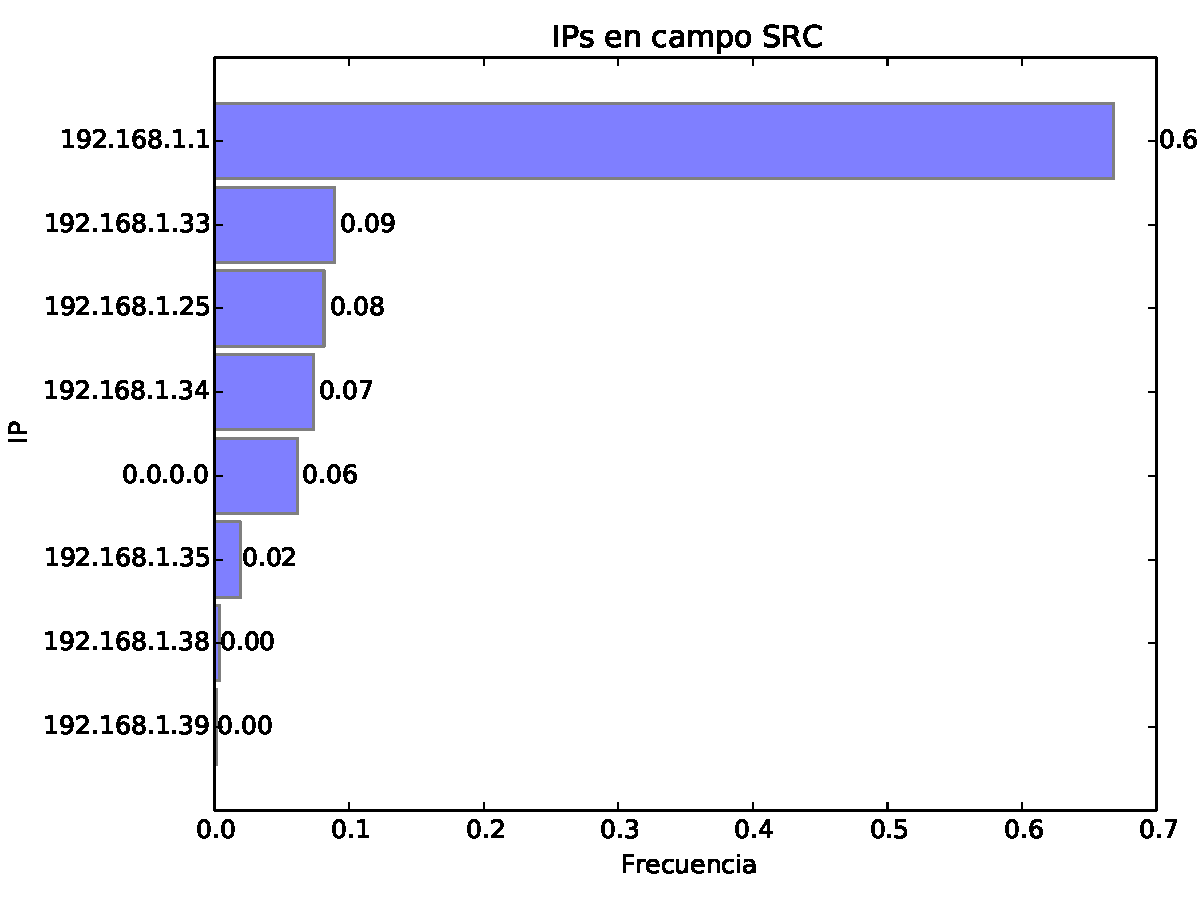
\includegraphics[width=1.0\textwidth]{resultados/casa/ipsSrc_1_6805902069.pdf}
		\caption{Estimaci\'on de la probabilidad de cada s\'imbolo en modelo SRC}
	\end{subfigure}
	~
	\begin{subfigure}{0.4\textwidth}
		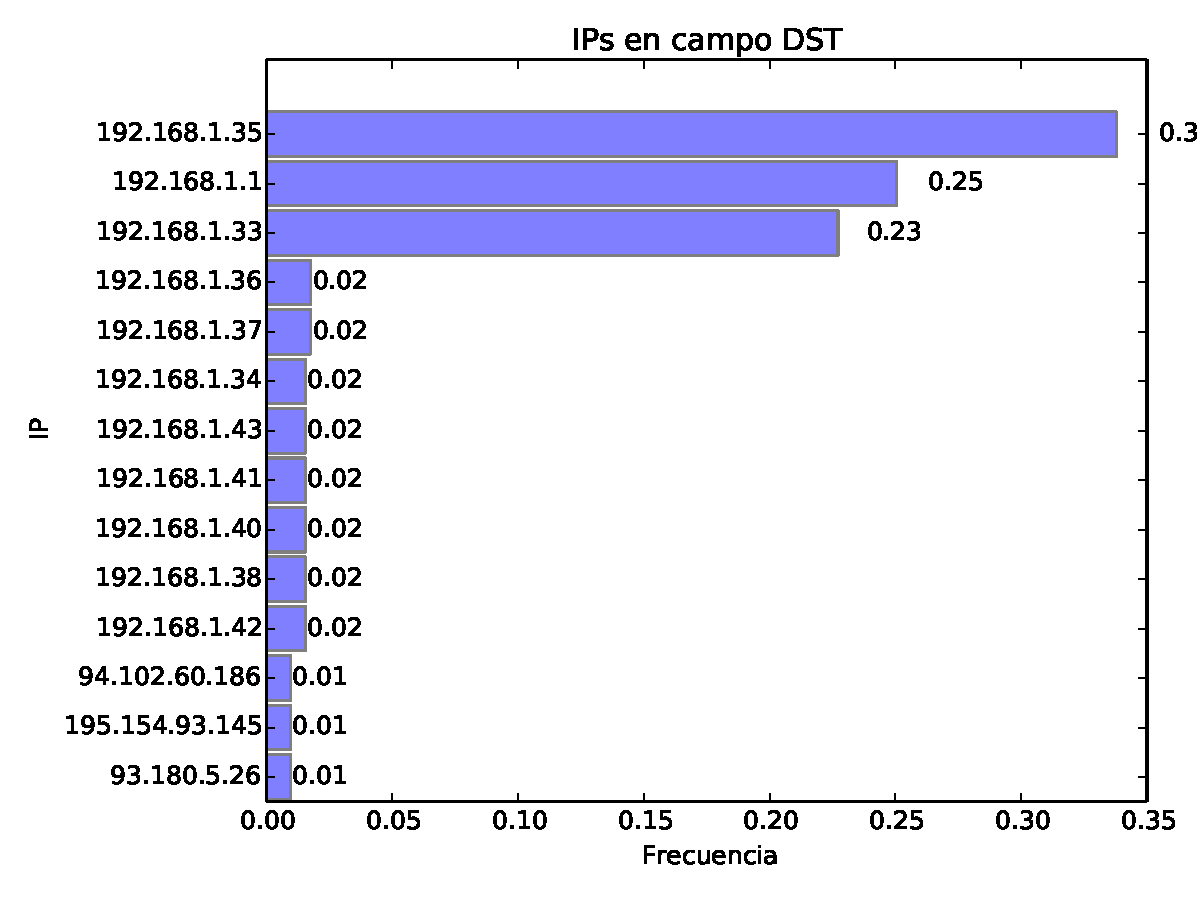
\includegraphics[width=1.0\textwidth]{resultados/casa/ipsDst_2_67355481854.pdf}
		\caption{Estimaci\'on de la probabilidad de cada s\'imbolo en modelo DST}
	\end{subfigure}
\end{figure}

\begin{wrapfigure}{R}{0.4\textwidth}
\vspace{-35pt}
\hspace{-35pt}
\centering
   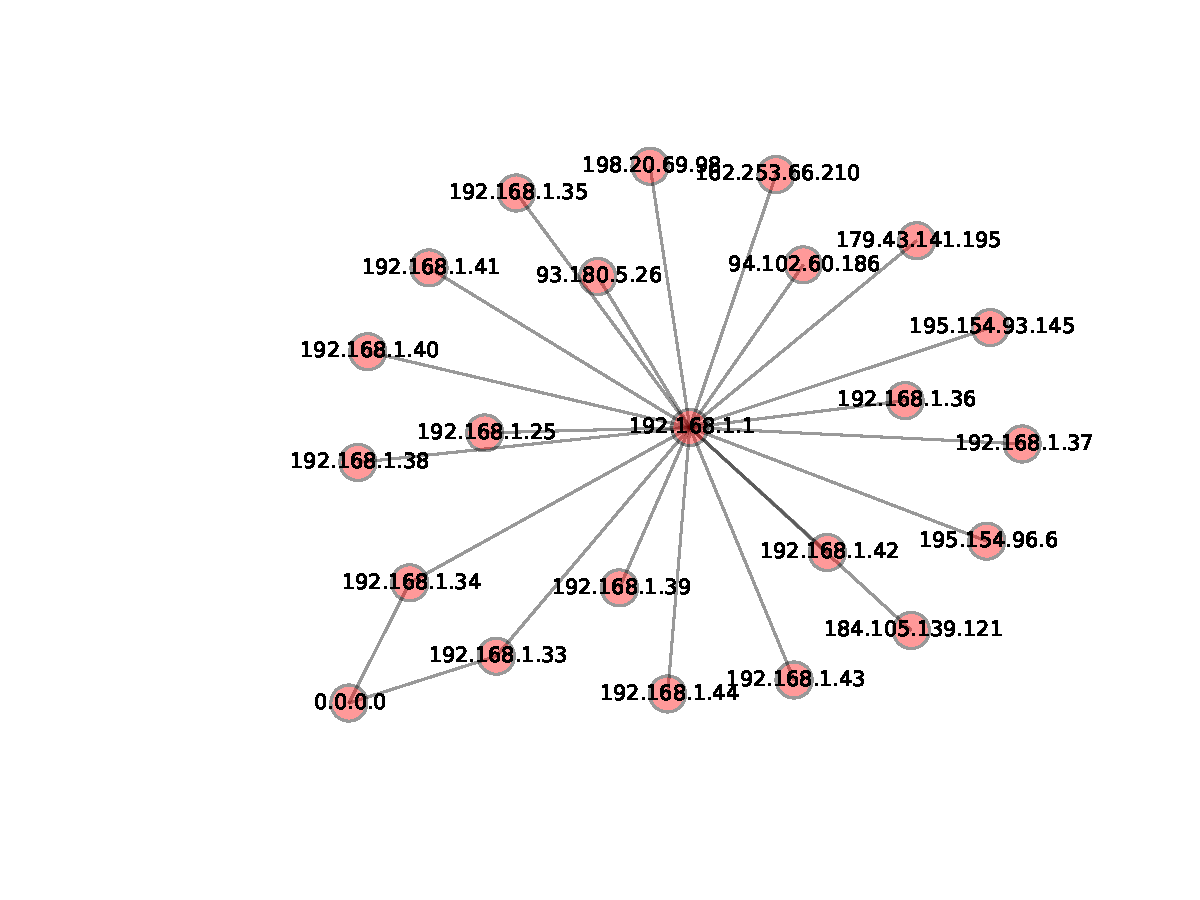
\includegraphics[width=0.4\textwidth]{resultados/casa/conectividadNX.pdf}
\vspace{-30pt}
   \caption{Grafo de la red}
\end{wrapfigure}

En el caso de la casa familiar sabíamos de antemano que el router es 192.168.1.1. Dicha ip es de las
que aparecen con mayor frecuencia en los campos SRC o DST. Ambos grafos presentan forma de estrella,
teniendo al router como centro. La entrop\'ia fue: $1.68$ para el modelo $SRC$ y $2.67$ para el modelo
DST. Cabe destacar que aunque no est\'a reflejado en los gr\'aficos, sucedi\'o algo interesante, 
aparecieron paquetes ARP con direcciones que no pertenecian a la red local, esto se puede deber a que
 \textcolor{red}{NO TENGO LA MENOR IDEA}



\begin{figure}[H]
   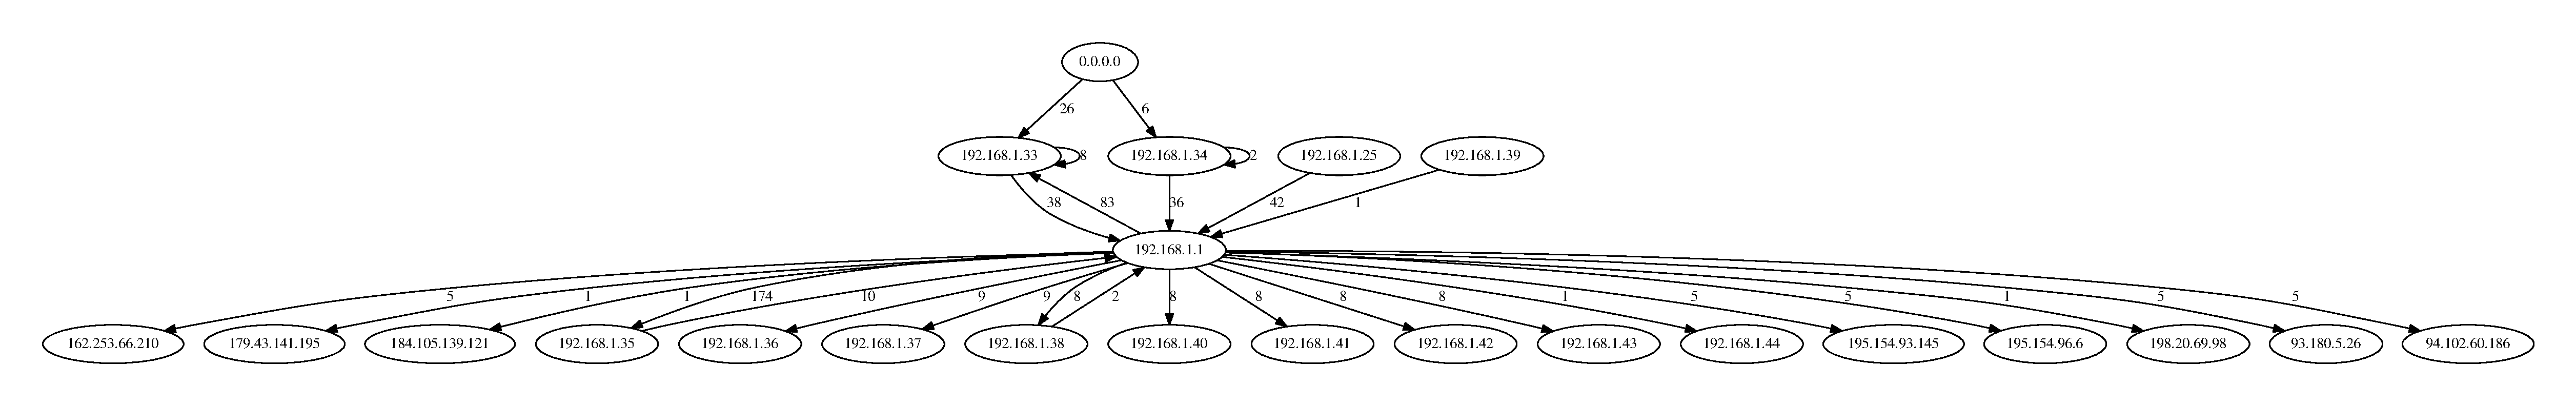
\includegraphics[width=1.0\textwidth]{resultados/casa/conectividad.pdf}
   \caption{Grafo dirigido de la red con peso en las aristas}
\end{figure}




*******************************************************************************************


~


Para el caso de la red abierta disponible en Starbucks, podemos ver en el 
grafo una notoria centralización de paquetes hacia/desde la dirección
10.254.88.1, lo cual sería el comportamiento esperado del router de la red
10.254.88.0/24. Asumimos que ésta es la dirección de la red puesto que 
la mayoría de las IPs de los paquetes capturados difieren en el último octeto.


Decimos "la mayoría" dado que se capturaron paquetes con direcciones que no 
parecen pertenecer a dicha red, a conocer:

\begin{itemize}
	\item Por un lado, el componente más pequeño, el cual se centraliza 
en la dirección 10.254.80.1. Suponemos que ésta dirección es la de un router
de otra red (10.254.80.0/24) y en algún momento sniffeamos paquetes de dicha 
red sin enterarnos.
	\item Por otro lado, la dirección 169.254.255.255. Investigamos esta
IP y encontramos que es utilizada como broadcast por DHCP que es un protocolo
de configuración automática de parámetros de red tales como direcciones IP
para interfaces y servicios.
	\item Por último, la dirección 0.0.0.0. \textcolor{red}{FALTA EXPLICAR y poner referencias}
\end{itemize} 


~


*******************************************************************************************


